\hypertarget{prototype-object}{%
\chapter{プロトタイプオブジェクト}\label{prototype-object}}\index{ぷろとたいぷおぶじぇくと@プロトタイプオブジェクト}
\thispagestyle{frontheadings}

「\href{../object/README.md}{オブジェクト}」の章では、オブジェクトの処理方法について見てきました。
その中で、空のオブジェクトであっても\texttt{toString}メソッドなどを呼び出せていました。

\begin{lstlisting}
const obj = {};
console.log(obj.toString()); // "[object Object]"
\end{lstlisting}

オブジェクトリテラルで空のオブジェクトを定義しただけなのに、\texttt{toString}メソッドを呼び出せています。
このメソッドはどこに実装されているのでしょうか?

また、JavaScriptには\texttt{toString}以外にも、オブジェクトに自動的に実装されるメソッドがあります。
これらのオブジェクトに組み込まれたメソッドを\textbf{\textgt{ビルトインメソッド}}\index{びるといんめそっど@ビルトインメソッド}と呼びます。

この章では、これらのビルトインメソッドがどこに実装され、なぜ\texttt{Object}のインスタンスから呼び出せるのかを確認していきます。
詳しい仕組みについては「\hyperlink{class}{クラス}」の章で改めて解説するため、この章では大まかな動作の流れを理解することが目的です。

\hypertarget{object-is-origin}{%
\section{\texorpdfstring{\texttt{Object}はすべての元}{Objectはすべての元}}\label{object-is-origin}}\index{Object@\texttt{Object}}

\texttt{Object}には、他の\texttt{Array}、\texttt{String}、\texttt{Function}などのオブジェクトとは異なる特徴があります。
それは、他のオブジェクトはすべて\texttt{Object}を継承しているという点です。

正確には、ほとんどすべてのオブジェクトは\texttt{Object.prototype}\index{Object.prototype@\texttt{Object.prototype}}プロパティに定義された\texttt{prototype}\index{prototype@\texttt{prototype}}オブジェクトを継承しています。
\texttt{prototype}オブジェクトとは、すべてのオブジェクトの作成時に自動的に追加される特殊なオブジェクトです。
\texttt{Object}の\texttt{prototype}オブジェクトは、すべてのオブジェクトから利用できるメソッドなどを提供するベースオブジェクトとも言えます。
\newpage
\begin{figure}[h]
\centering
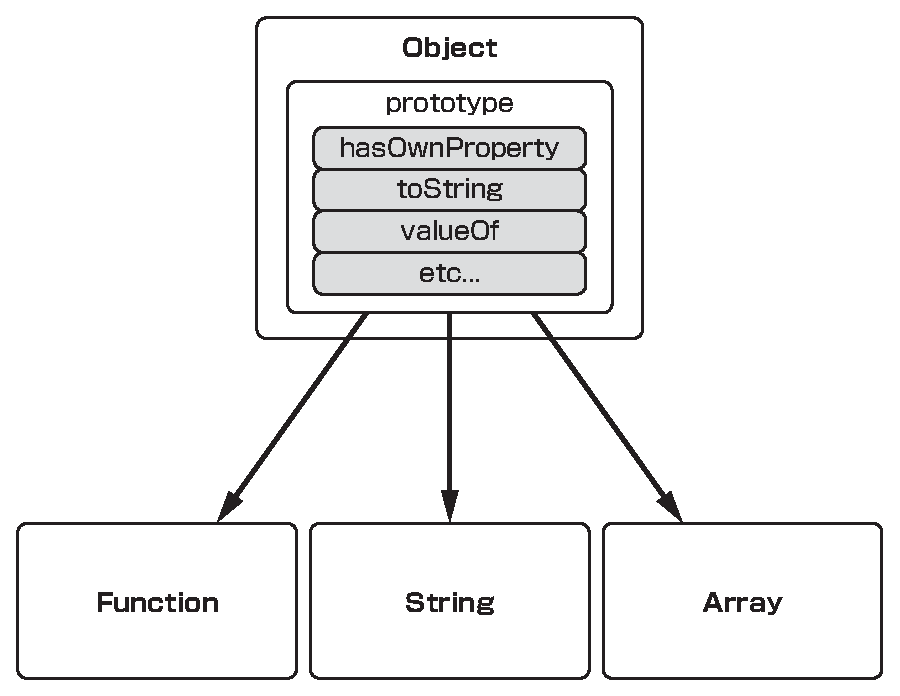
\includegraphics[width=90mm]{./fig/object-prototype.eps}
\caption{すべてのオブジェクトは\texttt{Object}の\texttt{prototype}を継承している}
\end{figure}

具体的にどういうことかを見てみます。

先ほども登場した\texttt{toString}\index{toString@\texttt{toString}}メソッドは、\texttt{Object}の\texttt{prototype}オブジェクトに定義があります。
次のように、\texttt{Object.prototype.toString}メソッドの実装自体も参照できます。

\begin{lstlisting}
// Object.prototypeオブジェクトにtoStringメソッドの定義がある
console.log(typeof Object.prototype.toString); // => "function"
\end{lstlisting}

このような\texttt{prototype}オブジェクトに組み込まれているメソッドは\textbf{\textgt{プロトタイプメソッド}}\index{ぷろとたいぷめそっど@プロトタイプメソッド}と呼ばれます。
この書籍では\texttt{Object.prototype.toString}のようなプロトタイプメソッドを「Objectの\texttt{toString}メソッド」と短縮して呼ぶことがあります。

\texttt{Object}のインスタンスは、この\texttt{Object.prototype}オブジェクトに定義されたメソッドやプロパティを継承します。
つまり、オブジェクトリテラルや\texttt{new Object}でインスタンス化したオブジェクトは、\texttt{Object.prototype}に定義されたものが利用できるということです。

次のコードでは、オブジェクトリテラルで作成(インスタンス化)したオブジェクトから、\texttt{Object.prototype.toString}メソッドを参照しています。
このときに、インスタンスの\texttt{toString}メソッドと\texttt{Object.prototype.toString}は同じものとなることがわかります。

\begin{lstlisting}
const obj = {
    "key": "value"
};
// objインスタンスはObject.prototypeに定義されたものを継承する
// obj.toStringは継承したObject.prototype.toStringを参照している
console.log(obj.toString === Object.prototype.toString); // => true
// インスタンスからプロトタイプメソッドを呼び出せる
console.log(obj.toString()); // => "[object Object]"
\end{lstlisting}

このように\texttt{Object.prototype}に定義されている\texttt{toString}メソッドなどは、インスタンス作成時に自動的に継承されるため、\texttt{Object}のインスタンスから呼び出せます。
これによりオブジェクトリテラルで作成した空のオブジェクトでも、\texttt{Object.prototype.toString}メソッドなどを呼び出せるようになっています。

このインスタンスから\texttt{prototype}オブジェクト上に定義されたメソッドを参照できる仕組みを\textbf{\textgt{プロトタイプチェーン}}\index{ぷろとたいぷちぇーん@プロトタイプチェーン}と呼びます。
プロトタイプチェーンの仕組みについては「\hyperlink{class}{クラス}」の章で扱うため、ここではインスタンスからプロトタイプメソッドを呼び出せるということがわかっていれば問題ありません。

\begin{tcolorbox}[enhanced jigsaw,breakable,title=\texttt{Object\#toString}という短縮した表記について]\label{prototype-shorthand-syntax}\index{Object\#toStringconst@\texttt{Object\#toString}}

この書籍では、\texttt{Object.prototype.toString}のように\texttt{prototype}を含めて毎回書くと冗長なため、「Objectの\texttt{toString}メソッド」と短縮して書く場合があります。
この書籍以外の文章では、\texttt{Object.prototype.toString}を\texttt{Object\#toString}のように\texttt{prototype}の代わりに\texttt{\#}を利用して表しているケースがあります。

\texttt{\#}\index{#@\texttt{\#}}が\texttt{prototype}の短縮表現として使われていたのは、\texttt{\#}がJavaScriptの構文として使われていない記号でもあったためです。
詳細は「\hyperlink{class}{クラス}」の章で解説しますが、ES2022では\texttt{\#}がJavaScriptの構文として追加され、\texttt{\#}という記号が意味を持つようになりました。
ES2022以降では、説明のために\texttt{\#}を\texttt{prototype}の短縮表現に使うと、人によっては異なる意味に見えてしまう可能性があります。

そのため、この書籍では\texttt{Object.prototype.toString}を\texttt{Object\#toString}のように\texttt{\#}を使って表す短縮表記は利用していません。
\end{tcolorbox}

\hypertarget{same-method-name-order}{%
\section{プロトタイプメソッドとインスタンスメソッドの優先順位}\label{same-method-name-order}}\index{いんすたんすめそっど@インスタンスメソッド}

プロトタイプメソッドと同じ名前のメソッドがインスタンスオブジェクトに定義されている場合もあります。
その場合には、インスタンスに定義したメソッドが優先して呼び出されます。

次のコードでは、\texttt{Object}のインスタンスである\texttt{customObject}に\texttt{toString}メソッドを定義しています。
実行してみると、プロトタイプメソッドよりも優先してインスタンスのメソッドが呼び出されていることがわかります。

\begin{lstlisting}
// オブジェクトのインスタンスにtoStringメソッドを定義
const customObject = {
    toString() {
        return "custom value";
    }
};
console.log(customObject.toString()); // => "custom value"
\end{lstlisting}

このように、インスタンスとプロトタイプオブジェクトで同じ名前のメソッドがある場合には、インスタンスのメソッドが優先されます。

\hypertarget{diff-in-operator-and-object-hasown}{%
\section{\texorpdfstring{\texttt{Object.hasOwn}静的メソッドと\texttt{in}演算子との違い}{Object.hasOwn静的メソッドとin演算子との違い}}\label{diff-in-operator-and-object-hasown}}\index{in@\texttt{in}}\index{Object.hasOwn@\texttt{Object.hasOwn}}

「\hyperlink{object}{オブジェクト}」の章で学んだ\texttt{Object.hasOwn}静的メソッドと\texttt{in}演算子の挙動の違いについて見ていきます。
2つの挙動の違いはこの章で紹介したプロトタイプオブジェクトに関係しています。

\texttt{Object.hasOwn}\index{Object.hasOwn@\texttt{Object.hasOwn}}静的メソッドは、指定したオブジェクト自体が指定したプロパティを持っているかを判定します。
一方、\texttt{in}演算子はオブジェクト自身が持っていなければ、そのオブジェクトの継承元である\texttt{prototype}オブジェクトまで探索して持っているかを判定します。
つまり、\texttt{in}演算子はインスタンスに実装されたメソッドなのか、プロトタイプオブジェクトに実装されたメソッドなのかを区別しません。

次のコードでは、空のオブジェクトが\texttt{toString}メソッドを持っているかを\texttt{Object.hasOwn}静的メソッドと\texttt{in}演算子でそれぞれ判定しています。
\texttt{Object.hasOwn}静的メソッドは\texttt{false}を返し、\texttt{in}演算子は\texttt{toString}メソッドがプロトタイプオブジェクトに存在するため\texttt{true}を返します。

\begin{lstlisting}
const obj = {};
// objというオブジェクト自体にtoStringメソッドが定義されているわけではない
console.log(Object.hasOwn(obj, "toString")); // => false
// in演算子は指定されたプロパティ名が見つかるまで親をたどるため、
// Object.prototypeまで見にいく
console.log("toString" in obj); // => true
\end{lstlisting}

次のように、インスタンスが\texttt{toString}メソッドを持っている場合は、\texttt{Object.hasOwn}静的メソッドも\texttt{true}を返します。

\begin{lstlisting}
// オブジェクトのインスタンスにtoStringメソッドを定義
const obj = {
    toString() {
        return "custom value";
    }
};
// オブジェクトのインスタンスがtoStringメソッドを持っている
console.log(Object.hasOwn(obj, "toString")); // => true
console.log("toString" in obj); // => true
\end{lstlisting}

\hypertarget{create-method}{%
\section{\texorpdfstring{オブジェクトの継承元を明示する\texttt{Object.create}メソッド}{オブジェクトの継承元を明示するObject.createメソッド}}\label{create-method}}\index{Object.create@\texttt{Object.create}}

\texttt{Object.create}メソッドを使うと、第一引数に指定した\texttt{prototype}オブジェクトを継承した新しいオブジェクトを作成できます。

これまでの説明で、オブジェクトリテラルは\texttt{Object.prototype}オブジェクトを自動的に継承したオブジェクトを作成していることがわかりました。
オブジェクトリテラルで作成する新しいオブジェクトは、\texttt{Object.create}メソッドを使うことで次のように書けます。

\begin{lstlisting}
// const obj = {} と同じ意味
const obj = Object.create(Object.prototype);
// objはObject.prototypeを継承している
// そのため、obj.toStringとObject.prototype.toStringは同じとなる
console.log(obj.toString === Object.prototype.toString); // => true
\end{lstlisting}

\hypertarget{inherit-object}{%
\section{ArrayもObjectを継承している}\label{inherit-object}}\index{Array}

\texttt{Object}と\texttt{Object.prototype}の関係と同じように、ビルトインオブジェクト\texttt{Array}も\texttt{Array.prototype}を持っています。
同じように、配列(\texttt{Array})のインスタンスは\texttt{Array.prototype}\index{Array.prototype@\texttt{Array.prototype}}を継承します。
さらに、\texttt{Array.prototype}は\texttt{Object.prototype}を継承しているため、\texttt{Array}のインスタンスは\texttt{Object.prototype}も継承しています。

\begin{lstlisting}
Arrayのインスタンス → Array.prototype → Object.prototype
\end{lstlisting}

\texttt{Object.create}メソッドを使って\texttt{Array}と\texttt{Object}の関係をコードとして表現してみます。
この疑似コードは、\texttt{Array}コンストラクタの実装など、実際のものとは異なる部分があるため、あくまでイメージであることに注意してください。

\begin{lstlisting}
// このコードはイメージです!
// Arrayコンストラクタ自身は関数でもある
const Array = function() {};
// Array.prototypeはObject.prototypeを継承している
Array.prototype = Object.create(Object.prototype);
// Arrayのインスタンスは、Array.prototypeを継承している
const array = Object.create(Array.prototype);
// arrayはObject.prototypeを継承している
console.log(array.hasOwnProperty === Object.prototype.hasOwnProperty); 
// => true
\end{lstlisting}

このように、\texttt{Array}のインスタンスも\texttt{Object.prototype}を継承しているため、
\texttt{Object.prototype}に定義されているメソッドを利用できます。

次のコードでは、\texttt{Array}のインスタンスから\texttt{Object.prototype.hasOwnProperty}メソッドが参照できていることがわかります。

\begin{lstlisting}
const array = [];
// Arrayのインスタンス -> Array.prototype -> Object.prototype
console.log(array.hasOwnProperty === Object.prototype.hasOwnProperty); 
// => true
\end{lstlisting}

\enlargethispage{\baselineskip}このような\texttt{hasOwnProperty}メソッドの参照が可能なのもプロトタイプチェーンという仕組みによるものです。

ここでは、\texttt{Object.prototype}はすべてのオブジェクトの親となるオブジェクトであることを覚えておくだけで問題ありません。
これにより、\texttt{Array}や\texttt{String}などのインスタンスも\texttt{Object.prototype}が持つメソッドを利用できる点を覚えておきましょう。

また、\texttt{Array.prototype}などもそれぞれ独自のメソッドを定義しています。
たとえば、\texttt{Array.prototype.toString}\index{Array.prototype.toString@\texttt{Array.prototype.toString}}メソッドもそのひとつです。
そのため、Arrayのインスタンスで\texttt{toString}メソッドを呼び出すと\texttt{Array.prototype.toString}が優先して呼び出されます。

\begin{lstlisting}
const numbers = [1, 2, 3];
// Array.prototype.toStringが定義されているため、Object.prototype.toStringとは
// 異なる出力形式となる
console.log(numbers.toString()); // => "1,2,3"
\end{lstlisting}

\hypertarget{not-inherit-object}{%
\section{\texttt{Object.prototype}を継承しないオブジェクト}\label{not-inherit-object}}\index{Object.prototype@\texttt{Object.prototype}}\index{Object.prototype@\texttt{Object.prototype}!けいしょうしない@継承しない}

\texttt{Object}はすべてのオブジェクトの親になるオブジェクトであると言いましたが、例外もあります。

イディオム(慣習的な書き方)ですが、\texttt{Object.create(null)}とすることで\texttt{Object.prototype}を継承しないオブジェクトを作成できます。
これにより、プロパティやメソッドをまったく持たない本当に\textbf{\textgt{空のオブジェクト}}を作れます。

\begin{lstlisting}
// 親がnull、つまり親がいないオブジェクトを作る
const obj = Object.create(null);
// Object.prototypeを継承しないため、hasOwnPropertyが存在しない
console.log(obj.hasOwnProperty); // => undefined
\end{lstlisting}

\texttt{Object.create}メソッドはES5から導入されました。
\texttt{Object.create}メソッドは\texttt{Object.create\newline (null)}というイディオムで、一部ライブラリなどで\texttt{Map}\index{Map@\texttt{Map}}オブジェクトの代わりとして利用されていました。
Mapとはキーと値の組み合わせを保持するためのオブジェクトです。

ただのオブジェクトもMapとよく似た性質を持っていますが、最初からいくつかのプロパティが存在し、アクセスできてしまいます。
なぜなら、\texttt{Object}のインスタンスはデフォルトで\texttt{Object.prototype}を継承するので、\texttt{toString}などのプロパティ名がオブジェクトを作成した時点で存在するためです。
そのため、\texttt{Object.create(null)}で\texttt{Object.prototype}を継承しないオブジェクトを作成し、そのオブジェクトが\texttt{Map}の代わりとして使われていました。

\begin{lstlisting}
// 空オブジェクトを作成
const obj = {};
// "toString"という値を定義してないのに、"toString"が存在している
console.log(obj["toString"]);// Function
// Mapのような空オブジェクト
const mapLike = Object.create(null);
// toStringキーは存在しない
console.log(mapLike["toString"]); // => undefined
\end{lstlisting}

しかし、ES2015からは本物の\texttt{Map}が利用できるため、\texttt{Object.create(null)}を\texttt{Map}の代わりに利用する必要はありません。
\texttt{Map}については「\hyperlink{map-and-set}{Map/Set}」の章で詳しく紹介します。

また\texttt{Object.create(null)}によって作成される空のオブジェクトは、\texttt{Object.hasOwn}静的メソッドがES2022で導入された理由でもあります。

次のように、\texttt{Object.prototype}を継承しないオブジェクトは、\texttt{Object.prototype.hasOwnProperty}メソッドを呼び出せません。
そのため、オブジェクトがプロパティを持っているかということを確認する際に、単純には\texttt{hasOwnProperty}メソッドが使えないという状況が出てきました。

\begin{lstlisting}
// Mapのような空オブジェクト
const mapLike = Object.create(null);
// Object.prototypeを継承していないため呼び出すと例外が発生する
console.log(mapLike.hasOwnProperty("key")); // => Error: hasOwnPropertyメソッドは
                                            // 呼び出せない
\end{lstlisting}

ES2022から導入された\texttt{Object.hasOwn}静的メソッドは、対象のオブジェクトが\texttt{Object.prototype}を継承していないかは関係なく利用できます。

\begin{lstlisting}
// Mapのような空オブジェクト
const mapLike = Object.create(null);
// keyは存在しない
console.log(Object.hasOwn(mapLike, "key")); // => false
\end{lstlisting}

このように、対象となるオブジェクトに依存しない\texttt{Object.hasOwn}静的メソッドは、\texttt{hasOwnProperty}メソッドの欠点を修正しています。

\hypertarget{conclusion}{%
\section{まとめ}\label{conclusion}}

この章では、プロトタイプオブジェクトについて学びました。

\begin{itemize}
\item
  プロトタイプオブジェクトはオブジェクトの作成時に自動的に作成される
\item
  \texttt{Object}のプロトタイプオブジェクトには\texttt{toString}などのプロトタイプメソッドが定義されている
\item
  ほとんどのオブジェクトは\texttt{Object.prototype}を継承することで\texttt{toString}メソッドなどを呼び出せる
\item
  プロトタイプメソッドとインスタンスメソッドではインスタンスメソッドが優先される
\item
  \texttt{Object.create}メソッドを使うことでプロトタイプオブジェクトを継承しないオブジェクトを作成できる
\end{itemize}

プロトタイプオブジェクトに定義されているメソッドがどのように参照されているかを確認しました。
このプロトタイプの詳しい仕組みについては「\hyperlink{class}{クラス}」の章で改めて解説します。
